%!TEX root=/home/ska124/Dropbox/Thesis/thes-full.tex
%% Copyright 1998 Pepe Kubon
%%
%% `05-introduction.tex' --- 1st chapter for thes-full.tex, thes-short-tex from
%%                the `csthesis' bundle

%%%%%%%%%%%%%%%%%%%%%%%%%%%%%%%%%%%%%%%%%%%%%%%%%
%
%       Chapter 1 
%
%%%%%%%%%%%%%%%%%%%%%%%%%%%%%%%%%%%%%%%%%%%%%%%%

\chapter{Introduction}
\label{introduction}

Cache memory systems are an integral part of computer architecture. Early mainframe computers in the 1960's were known to use a hierarchical cache memory organization. The first documented use of a data cache was in the IBM System/360 Model 85 \cite{liptay68}. \\

\begin{figure}[ht]
  %% Overview Cache Hierarchy
  \begin{center}
    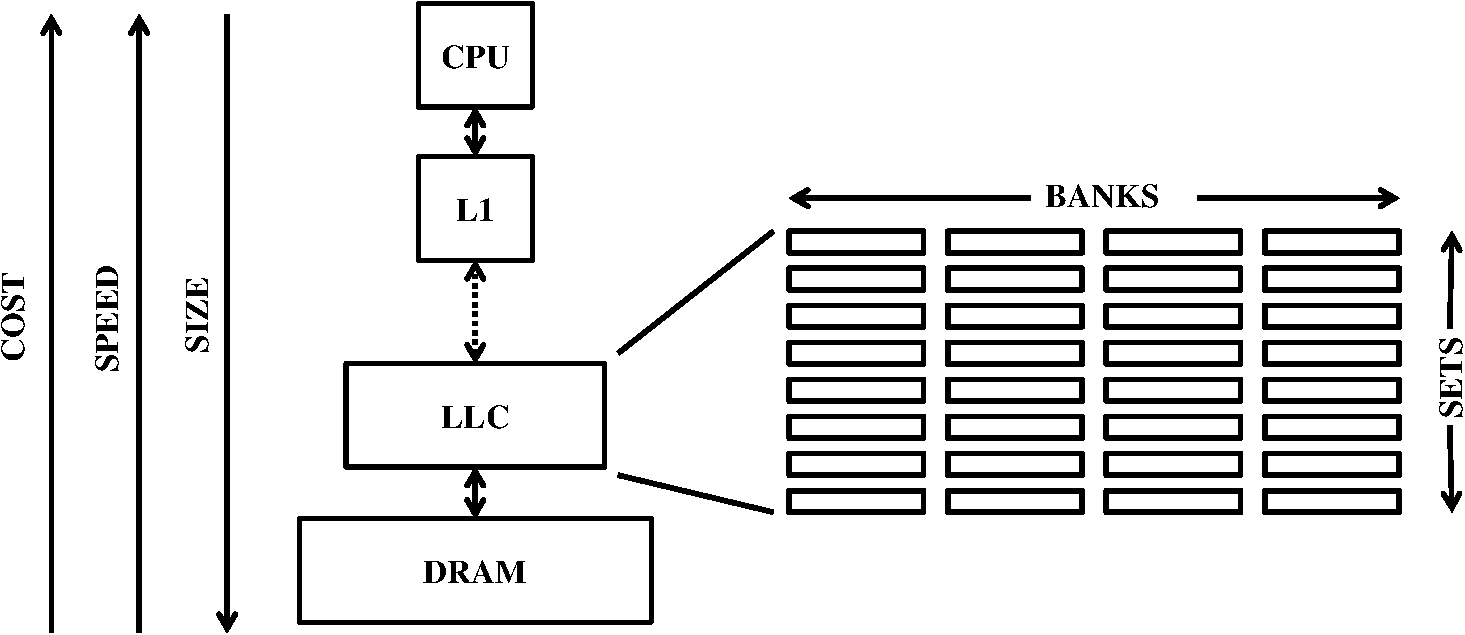
\includegraphics[width=\textwidth]{files/Figures/05-MemoryHierarchy.pdf}
    \caption[Canonical Memory Hierarchy]{\textbf{Canonical Memory Hierarchy} -- Moving down through the hierarchy, away from the processor, the levels are larger but slower. At each level the storage may be monolithic or sub divided in to "banks" for lower indexing overhead.}
    \label{fig:memory_hierarchy}
  \end{center}
\end{figure}

\section{Cache Memory Systems}
\label{sec:cache_memory_systems}
Most processors access data at the granularity of 4 to 8 bytes at a time. In order to exploit locality present in programs, caches are designed to retain small amounts of data close to the processor for fast access. The management of data in the cache is determined by a suitably selected replacement scheme. Caches are given designations to indicate their level in the memory hierarchy. The closest cached data stores to the processor are given lower numerical designations starting from \textit{L1} and increases as their distance from the processor increases. The last level of cache is often abbreviated as the \textit{LLC}. Each level in the cache hierarchy is linked in a daisy chain fashion, as shown in Fig \ref{fig:memory_hierarchy}, where there is an option for the data that is being cached to be replicated or not. The design choices can be enumerated as:

\begin{enumerate}
  \item Inclusive Caches : Lower level caches (further from the processor) replicate the cache lines present (although the data may be stale) present in the higher level caches. Inclusive caches can be found in Intel Sandy Bridge processors.
  \item Exclusive Caches : Caches lower in the hierarchy are guaranteed to not contain the cache lines present in the higher levels of the hierarchy. Present in the AMD architectures such as the Athlon processors.
  \item Non-Inclusive Caches : Also known as \textit{Non-Exclusive} or \textit{Accidentally Inclusive}, were used for a while in Intel architectures prior to the Intel P6. A lower level cache may or may not include a block cached at a higher level in the cache hierarchy.
\end{enumerate}

Caches are designed to take advantage of reuse of data by speeding up subsequent access to the same datum. They also speed up accesses to nearby data which may be fetched into the cache depending on its operating policy. The different types of locality which caches try to exploit can be enumerated as :

\begin{enumerate}
  \item Temporal Locality : Some applications tend to reuse the same data items over and over again during the course of their execution. This principle is the cornerstone for caching. Cache management policies usually implemented take into account the recency of data reuse to take a decision on what data is to be retained in the cache. Modern cache hierarchies implement a form of the \textit{Least Recently Used} algorithm to manage the contents of the cache.
  \item Spatial Locality : Due to conventional imperative programming paradigms, data is usually managed by grouping datum together in data structures, the fields of which are accessed in close proximity in the source code. Thus, in order to exploit this pattern, it is normal behavior for the cache to bring in a contiguous region, 32 -- 128 bytes in size, which contains the datum. The contiguous region of data brought into the cache is referred to as a \textit{cache block} or \textit{cache line}. The Intel Pentium 3 processors used a 32 byte line size which was increased to 64 bytes from Pentium 4. The IBM Power7 architectures use a 128 byte cache line where as the Intel Itanium2 uses a 64 bytes cache line size at the L1 and 128 byte cache line size at the L2 and L3.
\end{enumerate}

According to the place where a new cache line can be inserted into the cache, the cache can have varying associativity. If the policy requires that a certain block from memory can map only to a specific entry in the cache, it is known as a \textit{direct mapped} cache [Fig \ref{fig:cache_associativity}(a)]. On the other end of the spectrum, if a certain block from memory can map to any entry in the cache it is known as a \textit{fully associative} cache [Fig \ref{fig:cache_associativity}(c)].  It is easy to see that fully associative caches are the most flexible, however they incur significant costs in terms of latency and area overhead for standard cache operations. A cache look-up for a specific block is analogous to checking each item in a collection for a possible match. Conventional caches are organized as a 2-dimensional data structure where the rows are called \textit{sets}. Within each set there are a fixed number of cache blocks. The number of blocks in each set is the degree of associativity of the cache. Each possible entry in a set is called a \textit{way}. Thus a direct mapped cache has associativity of 1 where as a fully associative cache is one whose associativity is equal to the total number of cache blocks that the given cache can possibly hold.  


\begin{figure}[h]
  %% Get images from http://en.wikipedia.org/wiki/CPU_cache#Associativity
  \subfloat[Direct Mapped]{
    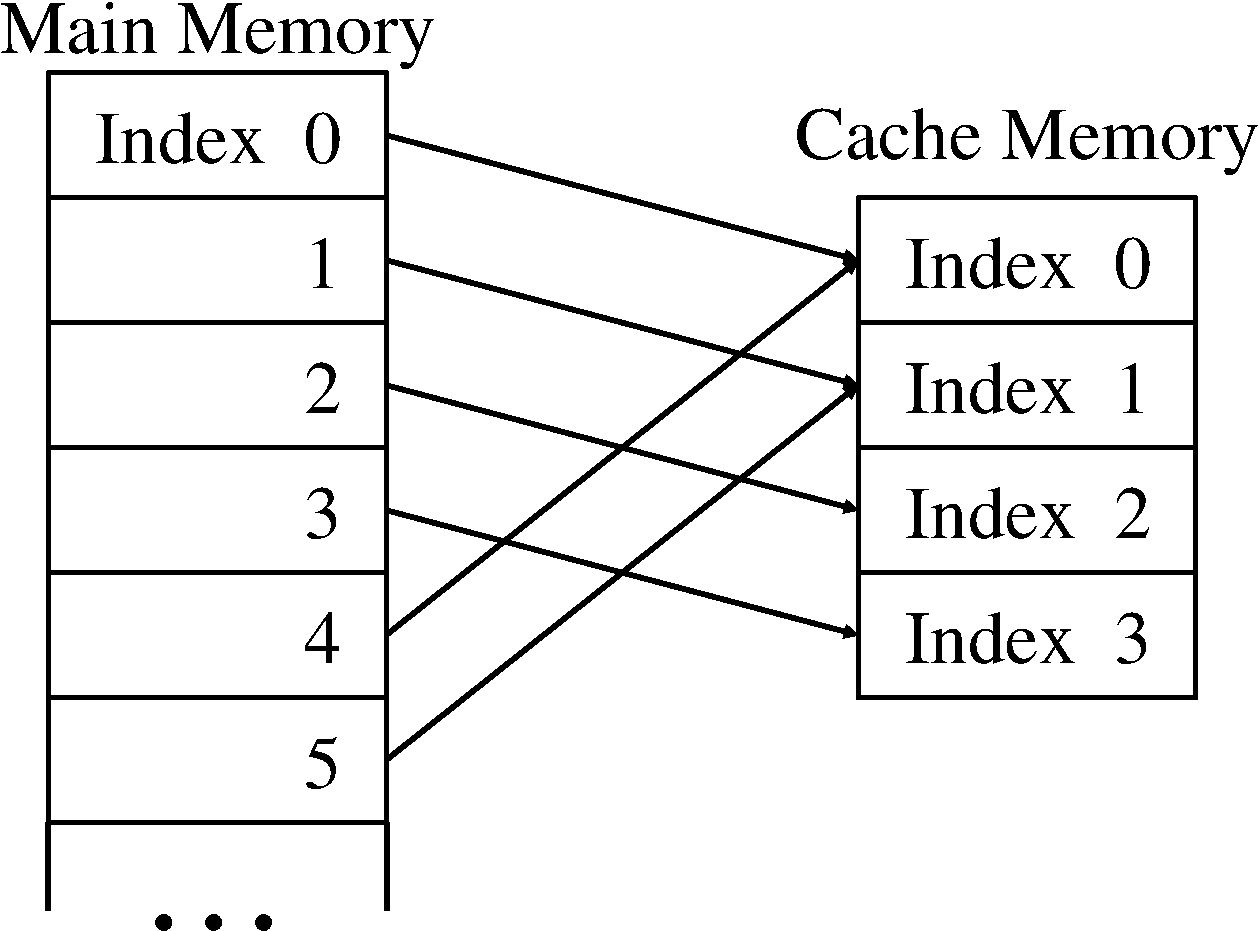
\includegraphics[width=0.32\textwidth]{files/Figures/05-DirectMapped.pdf}
  }
  \subfloat[2-way Set Associative ]{
     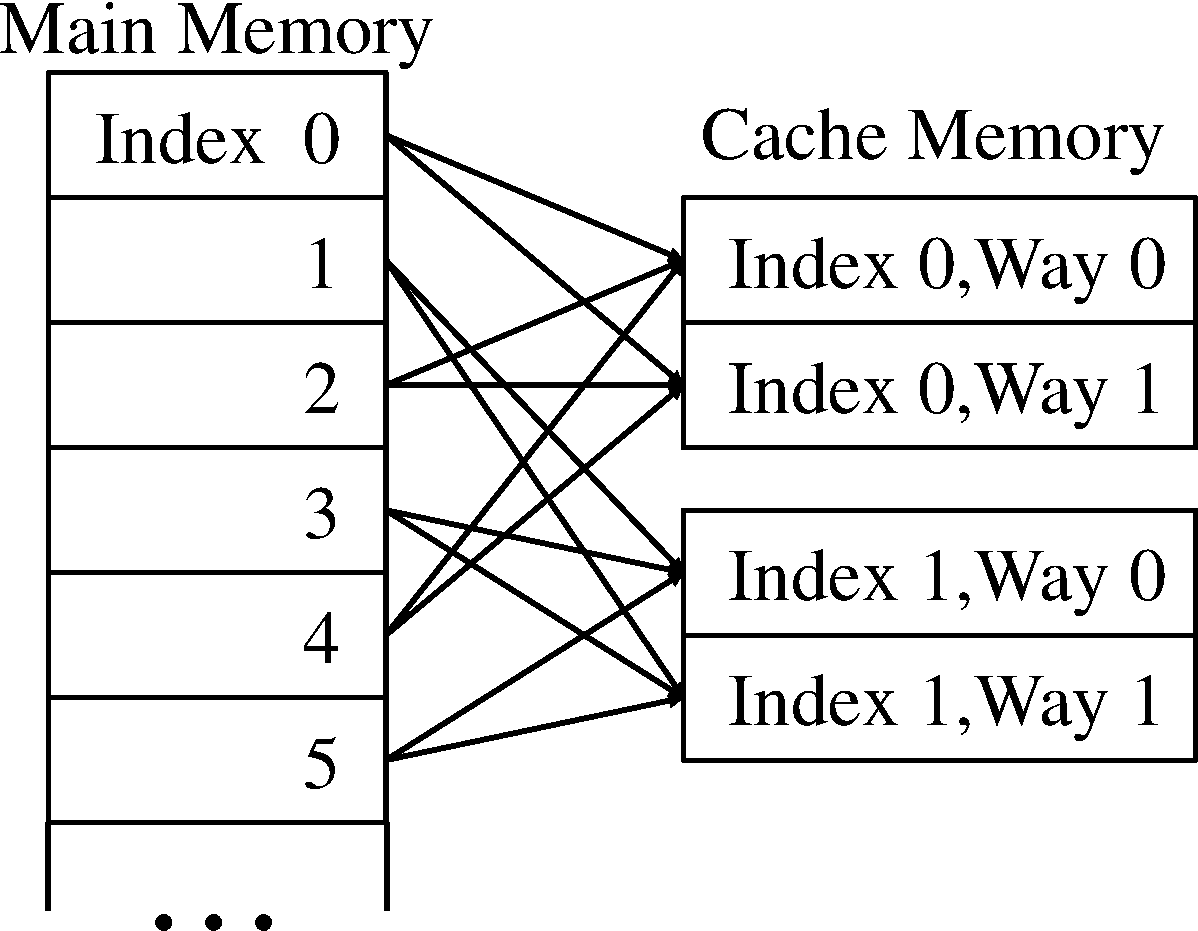
\includegraphics[width=0.32\textwidth]{files/Figures/05-2WayAssoc.pdf}
  }
  \subfloat[Fully Associative]{
     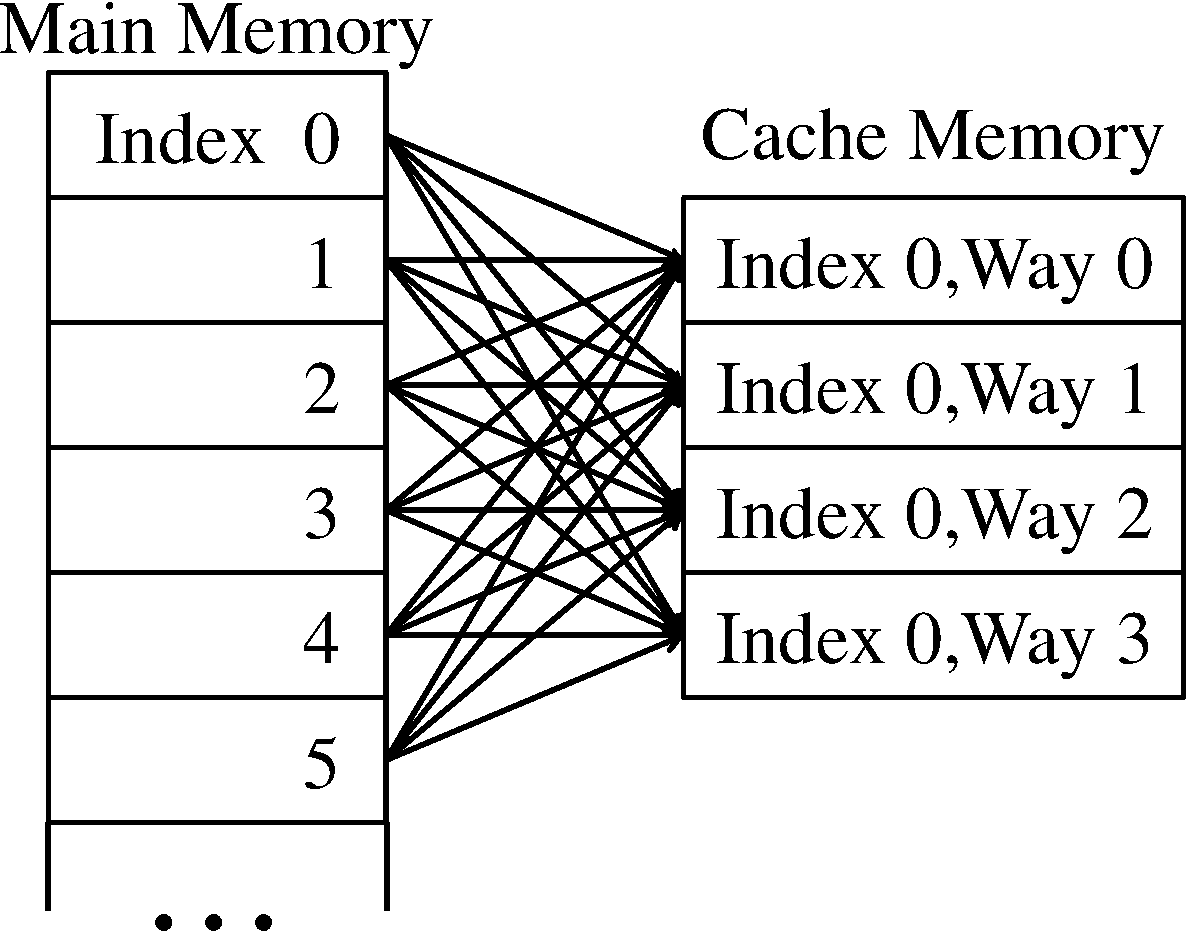
\includegraphics[width=0.32\textwidth]{files/Figures/05-FullAssoc.pdf}
  }
  \caption[Cache Associativity]{ Each block in memory maps to (a) a single entry (way) in the cache (b) one of 2 possible entries (ways) in the cache (c) any entry (way) in the cache}
  \label{fig:cache_associativity}
\end{figure}

\section{Motivation for change}

In conventional caches, the cache block defines the fundamental unit of data
movement and space allocation in caches. The blocks in the data array are
uniformly sized to simplify the insertion / removal of blocks, simplify cache
refill requests, and support low complexity tag organization. Unfortunately,
conventional caches are inflexible (fixed block granularity and fixed \# of
blocks) and caching efficiency is poor for applications that lack high spatial
locality.  Cache blocks influence multiple system metrics including bandwidth,
miss rate, and cache utilization. The block granularity plays a key role in
exploiting spatial locality by effectively prefetching neighboring words all
at once. However, the neighboring words could go unused due to the low
lifespan of a cache block. The unused words occupy interconnect bandwidth and
pollute the cache, which increases the \# of misses. We evaluate the influence
of a fixed granularity block below.

\subsection{Cache Utilization}

In the absence of spatial locality, multi-word cache blocks (typically 64
bytes on existing processors) tend to increase cache pollution and fill the
cache with words unlikely to be used.  To quantify this pollution, we segment
the cache line into words (8 bytes) and track the words touched before the
block is evicted.  We define utilization as the average \# of words touched in
a cache block before it is evicted. We study a comprehensive collection of
workloads from a variety of domains: 6 from PARSEC~\cite{Bienia:2008:PBS:1454115.1454128}, 7 from
SPEC2006, 2 from SPEC2000, 3 Java workloads from DaCapo~\cite{Blackburn:2006:DBJ:1167473.1167488}, 3
commercial workloads (Apache, SpecJBB2005, and TPC-C~\cite{Llanos:2006:TOT:1228268.1228270}), and the
Firefox web browser.  Subsets within benchmark suites were chosen based on
demonstrated miss rates on the fixed granularity cache (i.e., whose working
sets did not fit in the cache size evaluated) and with a spread and diversity
in cache utilization.  We classify the benchmarks into 3 groups
based on the utilization they exhibit: Low ($<$33\%), Moderate (33\%---66\%),
and High (66\%+) utilization (see Table~\ref{table:benchmark_categories}).

\begin{table}[!htb]
\vspace{-10pt}
\begin{center}
\caption{Benchmark Groups}
\label{table:benchmark_categories}
{
  \begin{tabular}{ |@{~}c@{~}|@{~}c@{~}|@{~}p{0.6\columnwidth}@{~}|}
    \hline
    Group & Utilization \% & Benchmarks \\
    \hline
    Low        & 0 --- 33\% & art, soplex, twolf, mcf, canneal, lbm, omnetpp \\
    \hline
    Moderate   & 34 --- 66\% & astar, h2, jbb, apache, x264, firefox, tpc-c, freqmine, fluidanimate \\
    \hline
    High       & 67 --- 100\% & tradesoap, facesim, eclipse, cactus, milc, ferret \\
    \hline
  \end{tabular}
 }
\end{center}
\end{table}
 %% Categories

\begin{figure}[!h]

 \centering
  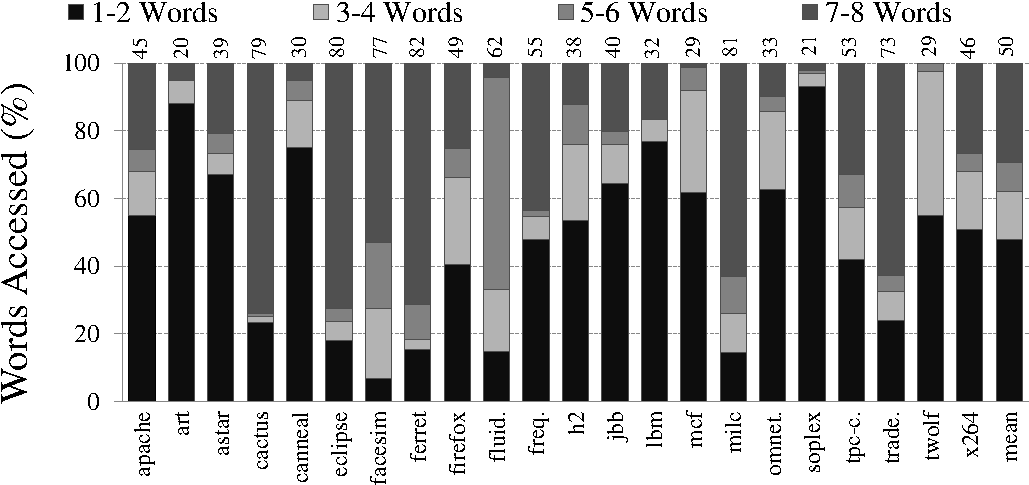
\includegraphics[width=\textwidth]{files/Plots/05-StackBar_Word_Access_64K.pdf}
  \caption[Distribution of words touched]{Distribution of words touched in a cache
    block. Avg. utilization is on top. (Config:
    64K, 4 way, 64-byte block.)}
  \label{fig:stackbar_words_64k}
\end{figure}

Figure~\ref{fig:stackbar_words_64k} shows the histogram of words touched at
the time of eviction in a cache line of a 64K, 4-way cache  (64-byte block, 8
words per block) across the different benchmarks.  Seven applications have
less than 33\% utilization and 12 of them are dominated ($>$50\%) by 1-2 word
accesses.  In applications with good spatial locality (cactus, ferret,
tradesoap, milc, eclipse) more than 50\% of the evicted blocks have 7-8 words
touched. Despite similar average utilization for applications such as astar
and h2 (39\%), their distributions are dissimilar; $\simeq$70\% of the blocks
in astar have 1-2 words accessed at the time of eviction,  whereas
$\simeq$50\% of the blocks in h2 have 1-2 words accessed per block.
Utilization for a single application also changes over time; for example,
ferret's  average utilization, measured as the average fraction of words used
in  evicted cache lines over 50 million instruction windows,  varies from 50\%
to 95\% with a periodicity of roughly 400 million instructions.

%Different temporal phases and 
%memory regions
%within an application may have different requirements: in firefox, 40\% of
%the blocks have 1--2 words touched, 26\% of the blocks have 3--4 words
%touched, and 34\% have 5+ words touched. 
%Overall, the utilization plot
%indicates the need for run time adjustment of cache block granularity.

\subsection{Causes of poor cache utilization}

Applications display poor cache utilization due to inefficient data structure access patterns. This could be due to 
\begin{enumerate}
  \item Programming practices : The array of structs (AoS) approach is a common programming practice. While performing computations upon the array if all elements of the struct are not referenced in close proximity, it could cause poor cache utilization. A relevant example can be seen in listing \ref{src:bscholes}.
  \item Incorrect assumptions about hardware : Hardware conscious code which attempts to optimize for cache behavior based on assumptions should be ported carefully. We found \textbf{streamcluster} of the PARSEC application suite, by default, attempt to optimize cache behavior for 32 byte cache line sizes. This finding was also reported by Liu and Berger\cite{Liu:2011:SPD:2048066.2048070}.
  \item Compiler directives : For better cache performance, sometimes compilers can attempt to allocate aligned blocks of memory. This functionality is exported to the programmer as \code{posix\_memalign} by \textit{GCC}, \code{\_\_aligned\_malloc} by \textit{MSVC} and \code{ippMalloc} by \textit{ICC}. These allocators may leave gaps filled with garbage values which are picked up by the cache when an entire line is fetched, thus reducing the effective caching capacity and reducing utilization.
  \item Interaction with cache geometry : Due to the set associative nature of conventional caches, a set can only contain a fixed number of ways. For instance, if a large amount of data is accessed in a strided fashion which happens to map to the same set, will cause evictions even though there may be space available for use in the other sets of the cache. This shortens the lifetime of the cache blocks in the selected set and may reduce utilization.
\end{enumerate}

\lstset{
  language=C++,
  % keywordstyle=\bfseries\ttfamily\color[rgb]{0,0,1},
  % identifierstyle=\ttfamily,
  % commentstyle=\color[rgb]{0.133,0.545,0.133},
  % stringstyle=\ttfamily\color[rgb]{0.627,0.126,0.941},
  showstringspaces=false,
  basicstyle=\small,
  numberstyle=\footnotesize,
  numbers=left,
  stepnumber=1,
  numbersep=10pt,
  tabsize=4,
  breaklines=true,
  prebreak = \raisebox{0ex}[0ex][0ex]{\ensuremath{\hookleftarrow}},
  breakatwhitespace=false,
  aboveskip={1.5\baselineskip},
  columns=fixed,
  %upquote=true,
  extendedchars=true,
  frame=single,
  frameround=tttt,
  captionpos=b,
  float=tb,
  boxpos=c,
  caption={Code snippet from the initialization phase of \textbf{blackscholes} benchmark from the PARSEC 2.1 \cite{Bienia:2008:PBS:1454115.1454128} application suite. The code references each \textit{OptionData} structure in the data array where the first 6 fields (24 bytes, as observed on a x86-64 machine with Ubuntu and gcc version 4.4.7) are referenced out of each struct which contains 9 fields (36 bytes). The problem is exacerbated as the \textit{OptionData} structure is allocated as a single chunk and is not cache aligned. The rest of the program demonstrates good cache behaviour.},
  % rulesepcolor=\color{black},
  % backgroundcolor=\color{lbcolor},
}

\noindent\begin{minipage}{\textwidth}
\begin{lstlisting}[label={src:bscholes}]
  /* blackscholes.c:354 */
  for (i=0; i<numOptions; i++) 
  {
      otype[i]      = (data[i].OptionType == 'P') ? 1 : 0;
      sptprice[i]   = data[i].s;
      strike[i]     = data[i].strike;
      rate[i]       = data[i].r;
      volatility[i] = data[i].v;
      otime[i]      = data[i].t;
  }
\end{lstlisting}
\end{minipage}

\begin{figure}[ht]

  \subfloat[64K - Low]{
    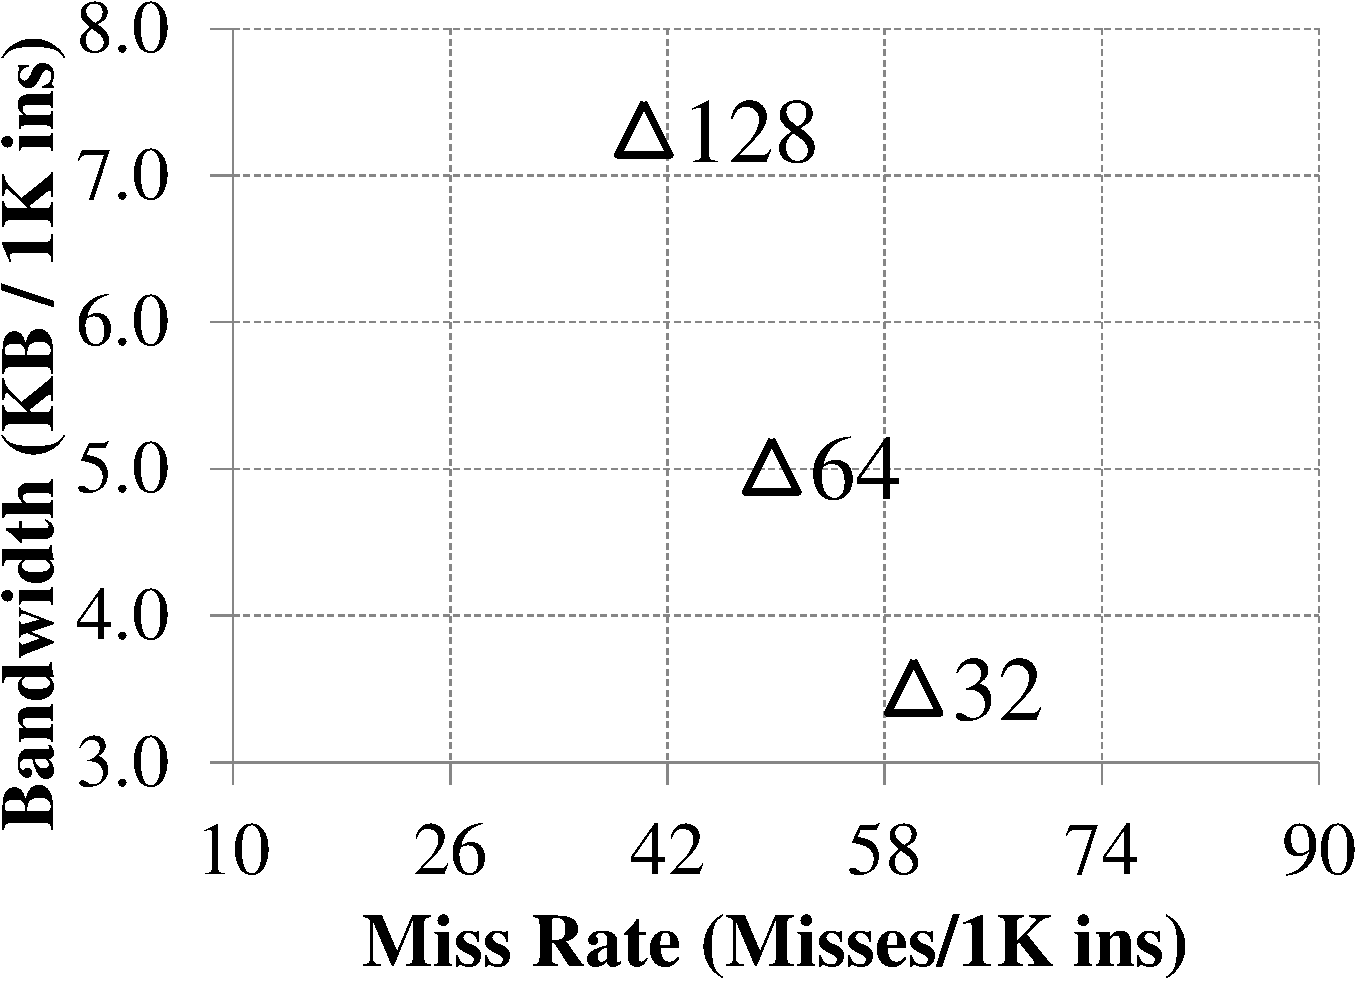
\includegraphics[width=0.48\textwidth]{files/Plots/05-Scatter_Bw_Miss_64K_low.pdf}
  }
  \subfloat[1M - Low]{
     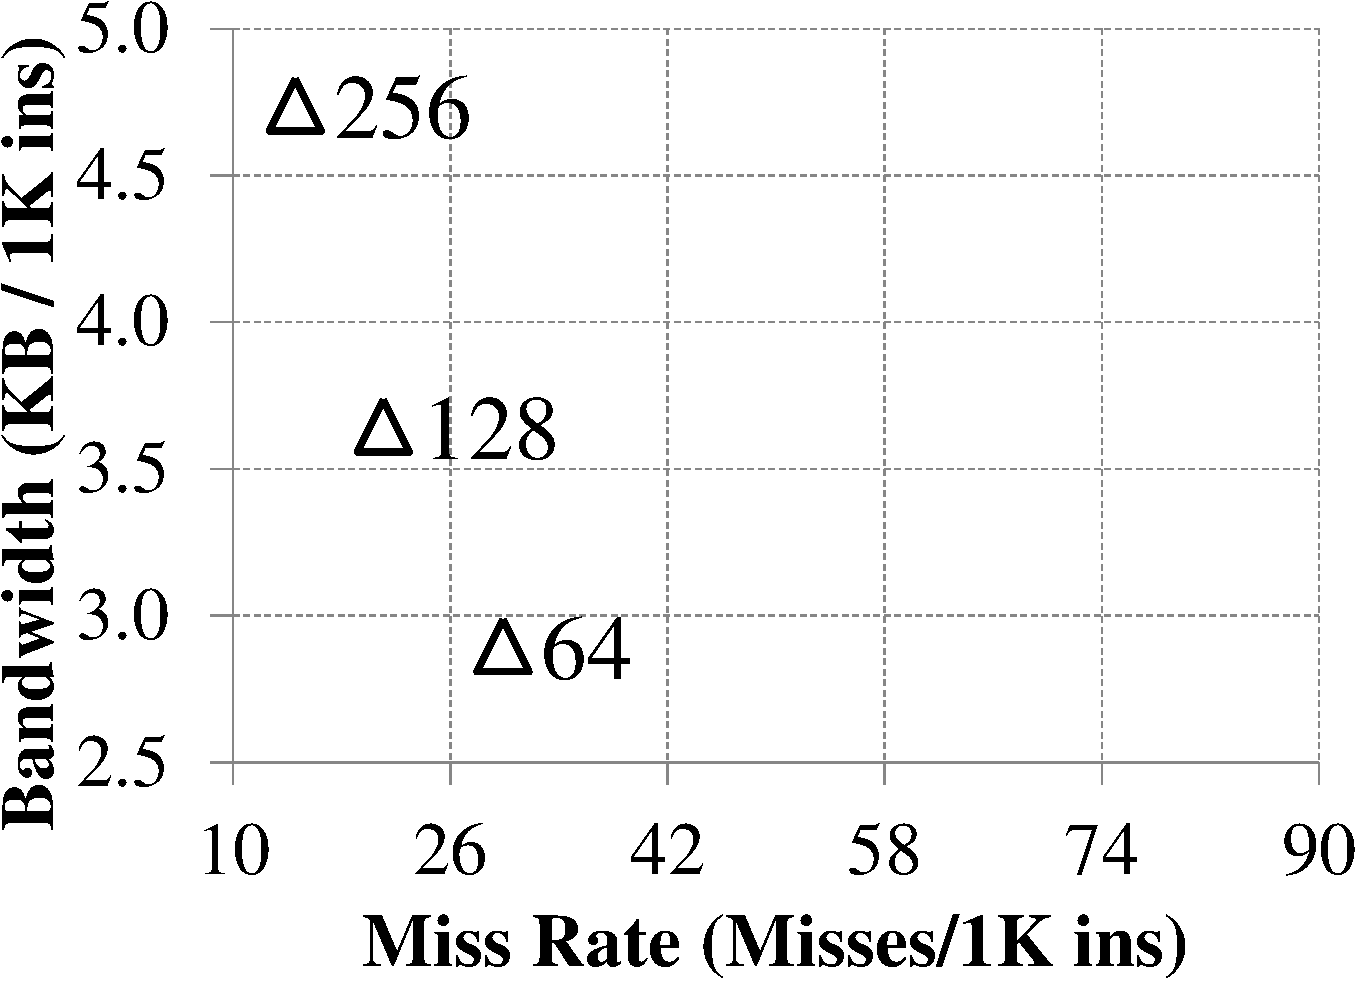
\includegraphics[width=0.48\textwidth]{files/Plots/05-Scatter_Bw_Miss_1M_low.pdf}
  }
  
  \subfloat[64K - Moderate]{
    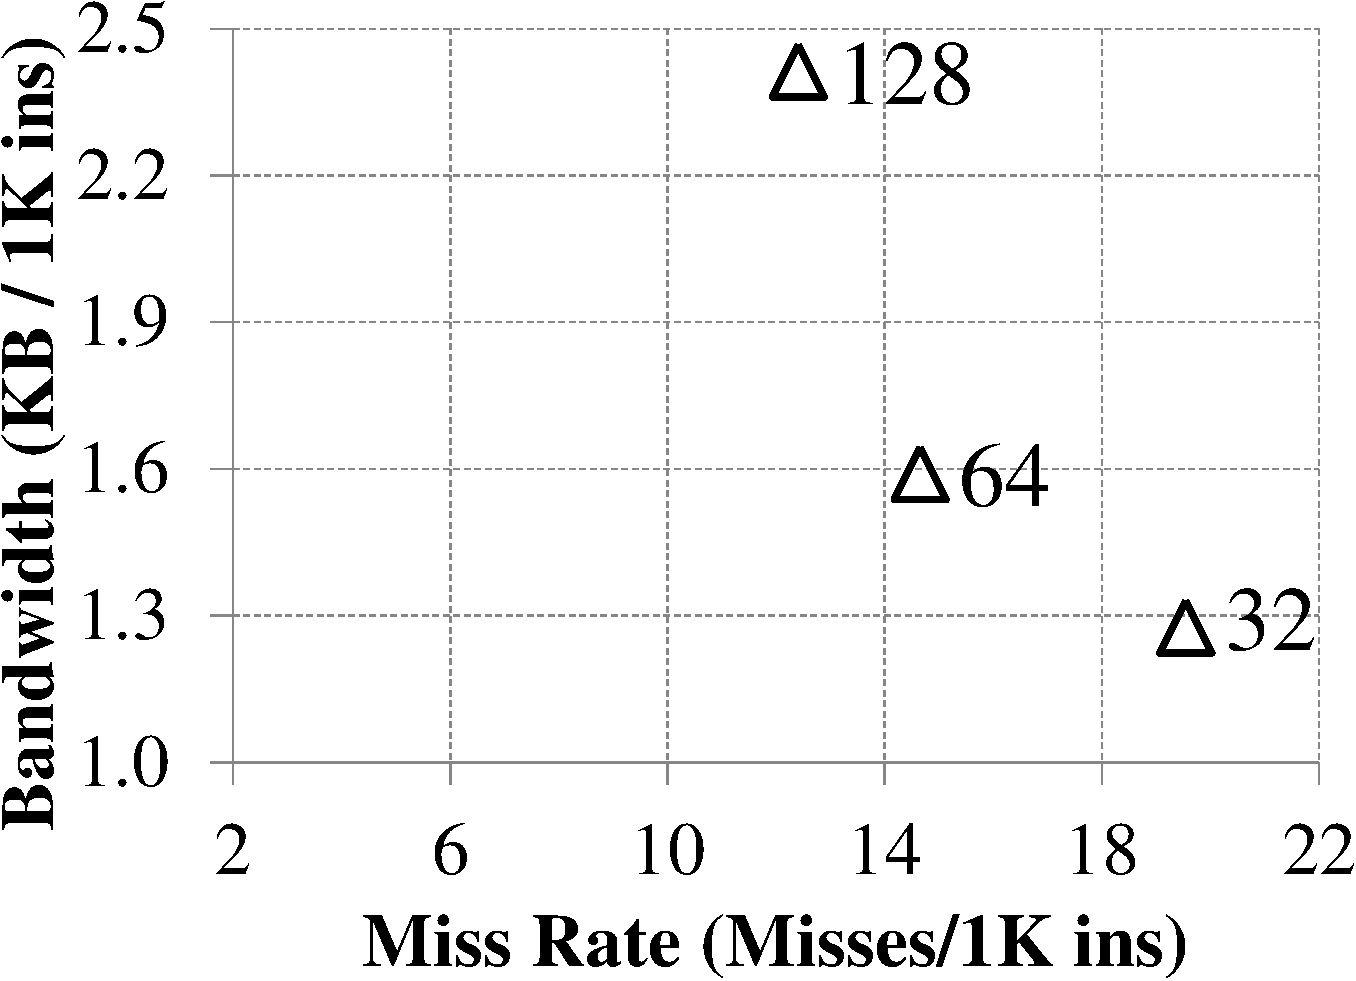
\includegraphics[width=0.48\textwidth]{files/Plots/05-Scatter_Bw_Miss_64K_mod.pdf}
  }
  \subfloat[1M - Moderate]{
     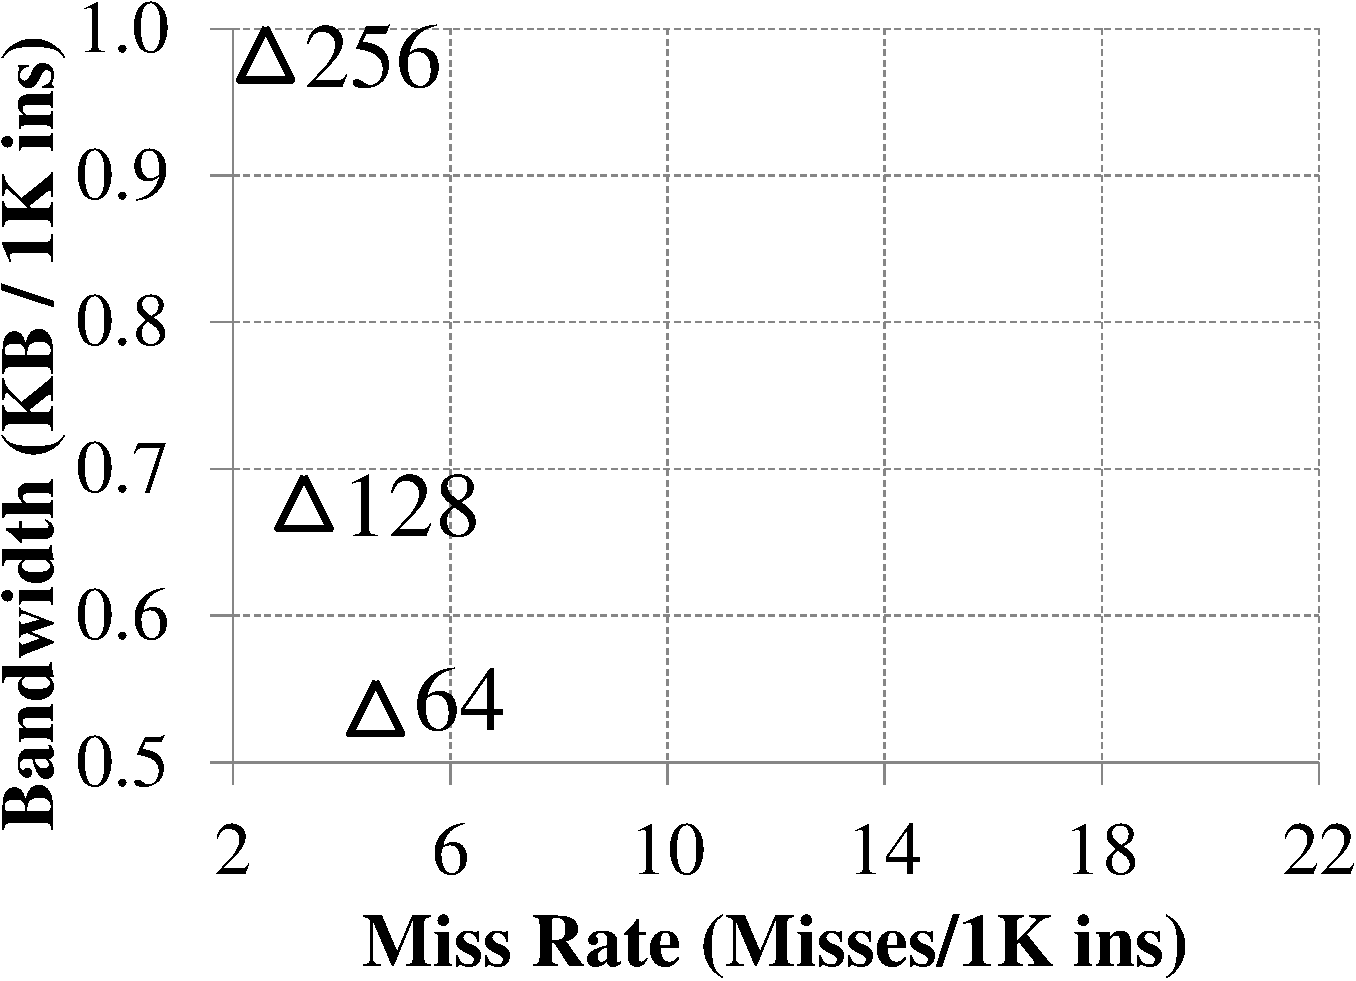
\includegraphics[width=0.48\textwidth]{files/Plots/05-Scatter_Bw_Miss_1M_mod.pdf}
  }
    
  \subfloat[64K - High]{
    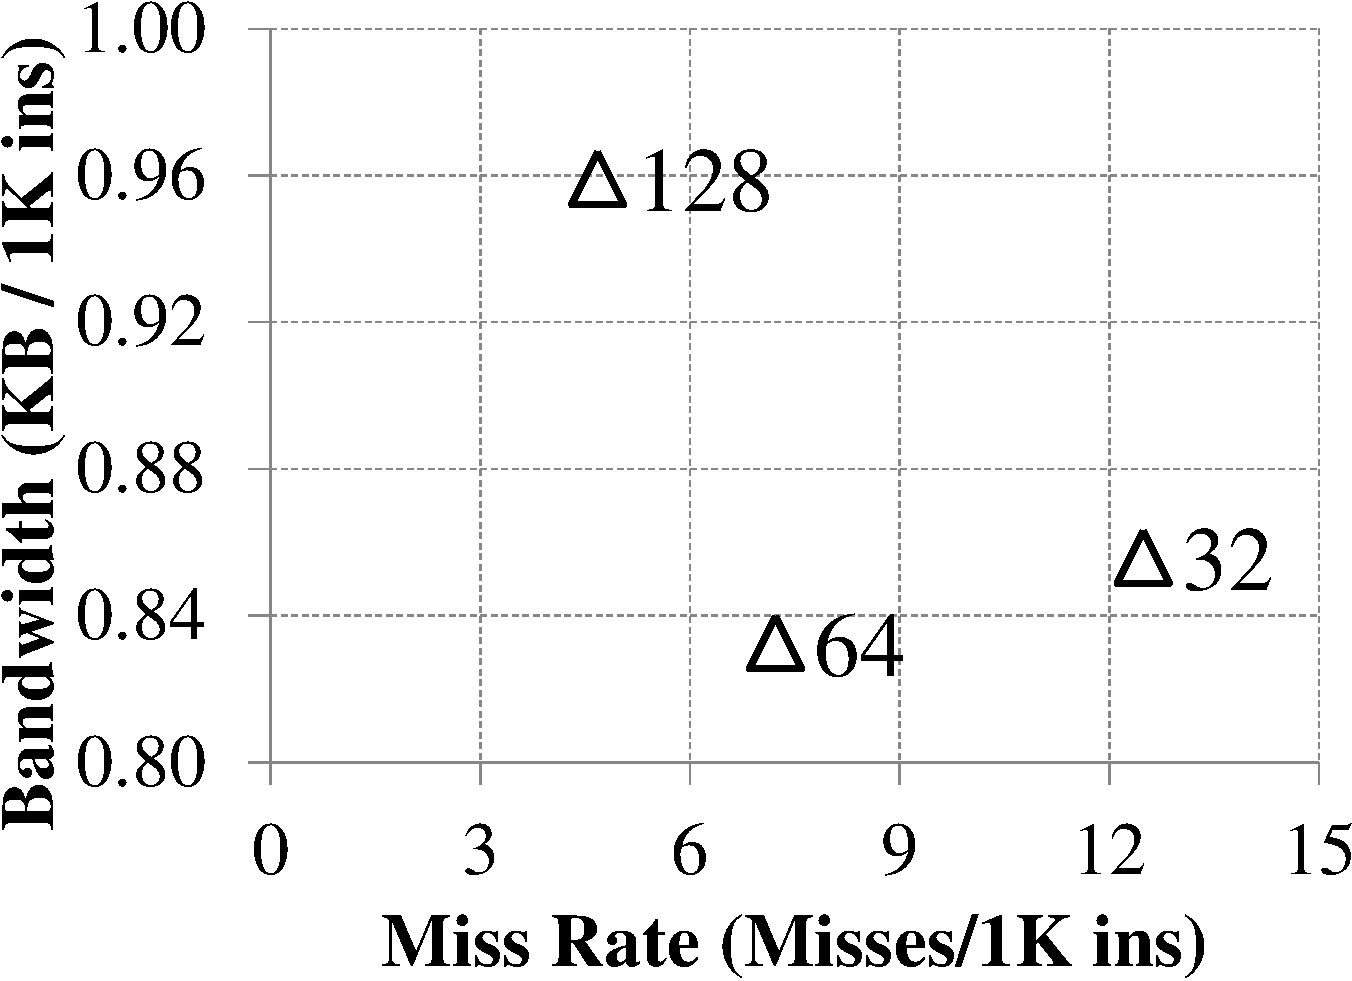
\includegraphics[width=0.48\textwidth]{files/Plots/05-Scatter_Bw_Miss_64K_high.pdf}
  }
  \subfloat[1M - High]{
     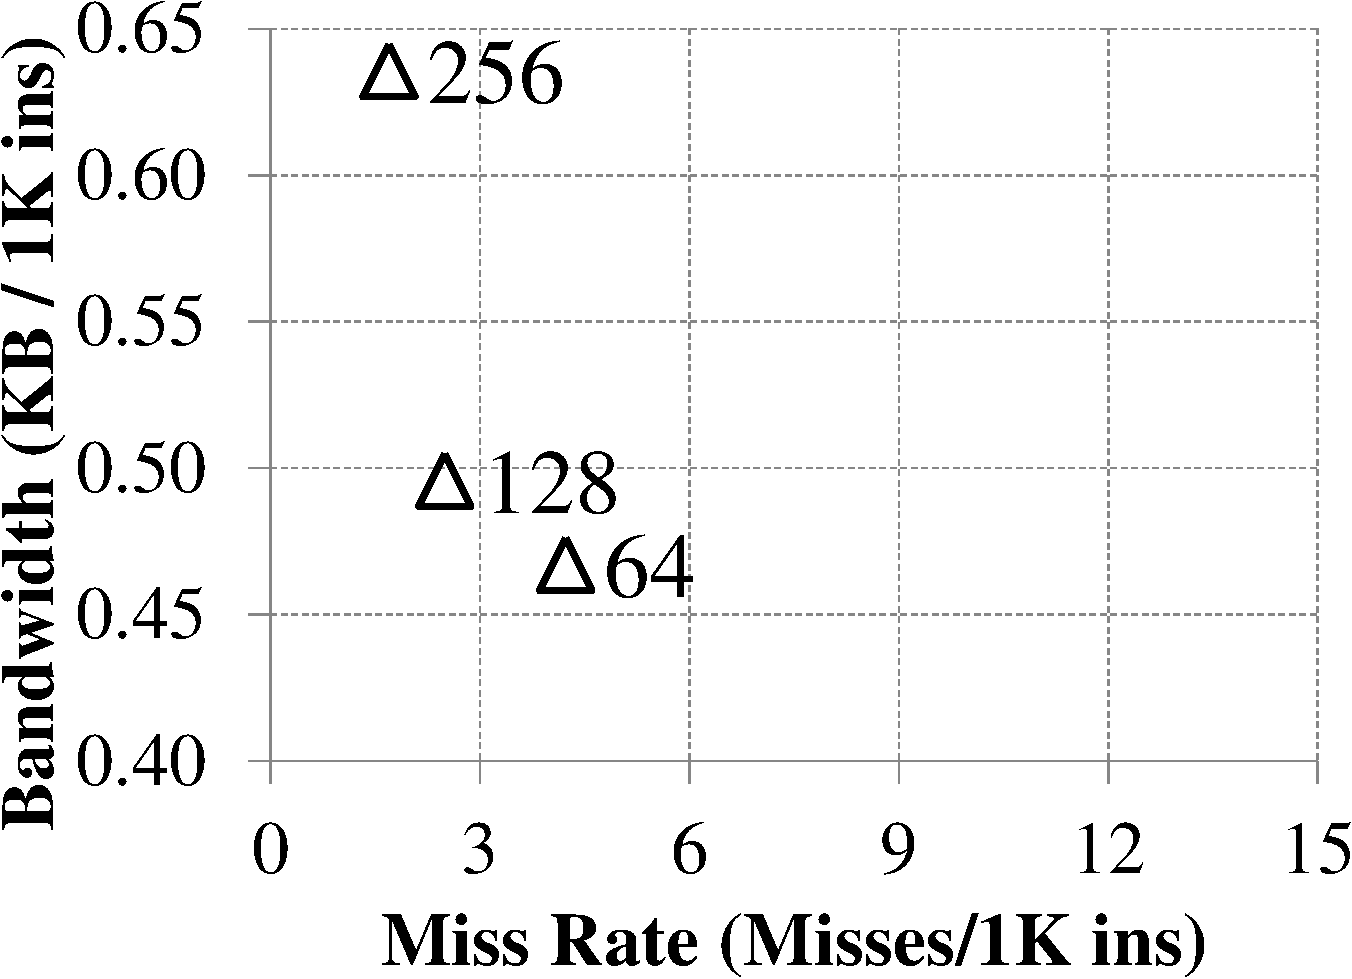
\includegraphics[width=0.48\textwidth]{files/Plots/05-Scatter_Bw_Miss_1M_high.pdf}
  }

  \caption[Bandwidth vs. Miss Rate]{Bandwidth vs. Miss Rate. (a),(c),(e): 64K, 4-way
    L1. (b),(d),(f): 1M, 8-way LLC.  Markers on the plot indicate cache
    block size. Note the different scales for different groups.}
  \label{fig:scatter_bw_64k_1m}
\end{figure}

\clearpage

\subsection{Effect of Block Granularity on Miss Rate and Bandwidth}

Cache miss rate directly correlates with performance, while under
current and future wire-limited technologies, bandwidth
directly correlates with dynamic energy.
Figure~\ref{fig:scatter_bw_64k_1m} shows the influence of block
granularity on miss rate and bandwidth for a 64K L1 cache and a 1M L2
cache keeping the number of ways constant. For the 64K L1, the plots
highlight the pitfalls of simply decreasing the block size to
accommodate the Low group of applications; miss rate increases by
2$\times$ for the High group when the block size is changed from 64B
to 32B; it increases by 30\% for the Moderate group. A smaller block
size decreases bandwidth proportionately but increases miss rate. With
a 1M L2 cache, the lifetime of the cache lines increases significantly, 
improving overall utilization. Increasing the block size from
64$\to$256 halves the miss rate for all application groups. 
The bandwidth is increased by 2$\times$ for the Low and Moderate.


\begin{table}[!h]
\caption{Optimal block size. Metric: $\mathbf{\frac{1}{Miss-rate \times Bandwidth}}$}
\label{table:bwmr_classify}
\begin{center}
{
\small
  \begin{tabular}{ |@{~}c@{~}| m{0.72\columnwidth} |}
    \hline
    \multicolumn{2}{|c|}{64K, 4-way} \\
    \hline
    Block  & Benchmarks \\
    \hline
    32B   & cactus, eclipse, facesim, ferret, firefox, fluidanimate,freqmine, milc, tpc-c, tradesoap \\
    \hline
    64B   &  art \\
    \hline
    128B  & apache, astar, canneal, h2, jbb, lbm, mcf, omnetpp, soplex, twolf, x264 \\
    \hline
    \multicolumn{2}{|c|}{1M, 8-way} \\
    \hline
    Block & Benchmarks \\
    \hline
    64B  & apache, astar, cactus, eclipse, facesim, ferret, firefox, freqmine, h2, lbm, milc, omnetpp, tradesoap, x264\\
    \hline
    128B & art\\
    \hline
    256B  & canneal, fluidanimate, jbb, mcf, soplex, tpc-c, twolf\\
    \hline
  \end{tabular}
}
\end{center}
\end{table}



Since miss rate and bandwidth have different optimal block
granularities, we use the following metric: $\frac{1}{Miss Rate \times
  Bandwidth}$ to determine a fixed block granularity suited to an
application that takes both criteria into account.
Table~\ref{table:bwmr_classify} shows the block size that maximizes
the metric for each application.  It can be seen that different
applications have different block granularity requirements.  For
example, the metric is maximized for apache at 128 bytes and for
firefox (similar utilization) at 32 bytes.  Furthermore, the optimal
block sizes vary with the cache size as the cache lifespan
changes. This highlights the challenge of picking a single block size
at design time especially when the working set does not fit in the
cache.
%In short, \textit{the tradeoff between increasing the 
%  cache block granularity to achieve spatial prefetching and lower miss rate, 
%  and reducing the granularity to minimize traffic and pollution needs
%  adaptive cache blocks.}

\subsection{Need for adaptive cache blocks}
Our observations motivate the need for adaptive cache line
granularity that matches the spatial locality of the data access patterns
in an application. In summary:
\begin{itemize}
  \item  Smaller cache lines improve utilization but tend to increase
    miss rate and potentially traffic for applications with good
    spatial locality, affecting the overall performance.
  \item Large cache lines pollute the cache space and interconnect
    with unused words for applications with poor spatial locality, 
   significantly decreasing the caching efficiency.
  \item Many applications waste a significant fraction of the cache
  space. Spatial locality varies not only across applications but also
  within each application, for different data structures as well as 
  different phases of access over time.   

%\item Optimizing miss rate (impacts performance), bandwidth (impacts
%  dynamic energy), and utilization simultaneously with a fixed size
%  cache line is not tractable, since in many cases the optimality is
%  achieved at different block sizes.
\end{itemize}


\section{Dissertation Outline}

Chapter \ref{chap:ac_architecture} describes the \AC\ architecture whilst comparing it with conventional architecture and looking at related work. The hardware complexity, implementation issues and simulator infrastructure are discussed in Chapter \ref{chap:hardware_complexity_and_simulation}. The experimental results of an exhaustive evaluation of the \AC\ is presented in Chapter \ref{chap:evaluation}. Conclusions and future work are outlined in Chapter \ref{chap:conclusions}.
